\section{1. Descripción técnica-conceptual del proyecto a realizar}
\label{sec:descripcion}

Para productos de ámbitos espaciales, como lo son los satélites, muchas veces es difícil, y en ocasiones imposible, generar escenarios realistas para pruebas de los elementos que lo componen. Ya sea por no poder generar las mismas condiciones ambientales, o porque la naturaleza de la maniobra que se busca probar implicaría un daño a los equipos bajo revisión.

En este contexto, es común replicar los elementos de interés de manera programada cumpliendo con cierto grado de representación. De manera tal que se comporten de la manera más similar posible a su contraparte física. Dichos elementos desarrollados se los llaman emulados o simulados. Uno de los componentes que se suele tener mayor interés en simular es el procesador de la computadora a bordo.

El término Computadora a Bordo (OBC, por las siglas en inglés de On Board Computer) suele referirse a la unidad en la que se ejecuta el Software A Bordo (OBSW, por sus siglas en inglés de On Board Software) y su rol principal es el control de los subsistemas del satélite. Esto incluye recolectar información de diferentes subsistemas, analizarla y tomar las decisiones y acciones apropiadas cuando sea requerido.

Dentro de la OBC se encuetra un microprocesador, dicho componente es el elemento de interés para el presente trabajo. Siendo el elemento a desarrollar.

Cabe destacar, que hoy en día existen emuladores tanto de código abierto como privativos para distintos microprocesadores. Un ejemplo claro de emulador de código abierto es Qemu, que abarca un amplio abanico de microprocesadores, entre ellos, algunos utilizables en el ámbito espacial.

Cada caso de emulador, aunque solucionan el problema en cuestión, viene con sus respectivas desventajas. Por ejemplo, los emuladores de código abierto suelen divergir para ampliar el rango de procesadores soportados, generalmente disminuyendo su performance. Por otro lado, los emuladores privativos al no tener acceso al código muchas veces se vuelven difíciles de integrar, ya que no se tiene un conocimiento exacto sobre sus limitaciones, y en general, difíciles de depurar el software que ejecutan.

Bajo estas premisas se plantea crear un emulador de microprocesador Leon3 para desarrollo de software satelital y simuladores. Al ser un desarrollo a medida, se tendrá la ventaja de la no-diversificación del procesador, es decir, estará únicamente orientado a un solo microprocesador. Esperando una ganancia en performance comparado con su contraparte de código abierto. Al mismo tiempo, se tendrá un conocimiento extenso del alcance y limitaciones de las capacidades del software en cuestión. Haciendo, de esta manera, más simple la integración y depuración en su uso.

%%% Corrected with grammarly up-to here
















\begin{consigna}{red} % El bloque "consigna" se usa para poner texto en rojo y dar una pequeña ayuda sobre cómo completar la sección. En cada entrega parcial deben eliminar los comandos begin y end del bloque consigna de las secciones que hayan completado.

El objetivo es que el lector en una o dos páginas entienda de qué trata el proyecto y cuáles son sus desafíos, cuál es la motivación para realizarlo y su importancia.

Se debe introducir el contexto del proyecto, el estado del arte en la temática, describir la propuesta de valor, cúal es el problema que atiende y cuál es la solución que se propone. Se debe dar una descripción funcional de la solución que incluya un diagrama en bloques.

Puede ser útil incluir en esta sección la respuesta a alguna de estas preguntas:

\begin{itemize}
	\item ¿Cuál es el contexto del proyecto, es un emprendimiento personal, un proyecto para una empresa, es parte del programa de vinculación con empresas del posgrado?
	\item ¿Existen o aplican condiciones especiales al proyecto, financiamiento de algún programa público o privado, acuerdos de confidencialidad, acuerdos sobre la propiedad intelectual de los entregables u otros?
	\item ¿Cómo se compara la solución propuesta con el estado del arte en el campo de aplicación? ¿En qué aspectos destaca?
	\item ¿Ayuda a la explicación si se incluye un lienzo Canvas del Modelo de Negocio?
	\item ¿En qué estado del ciclo de vida está la solución que se propone?
	\item ¿Cuáles son las características del cliente (el adoptante de los entregables del proyecto) qué valora, qué necesita?
	\item ¿Por dónde pasa la innovación?
\end{itemize}

La descripción técnica-conceptual \textbf{debe incluir al menos un diagrama en bloques del sistema} y descripción funcional de la solución propuesta.

Las figuras se deben mencionar en el texto ANTES de que aparezcan con una frase como la siguiente: ``En la Figura \ref{fig:diagBloques} se presenta el diagrama en bloques del sistema. Se observa que...''.  La regla es que las figuras nunca pueden ir antes de ser mencionadas en el texto, porque sino el lector no entiende por qué de pronto aparece una figura.

\begin{figure}[htpb]
\centering
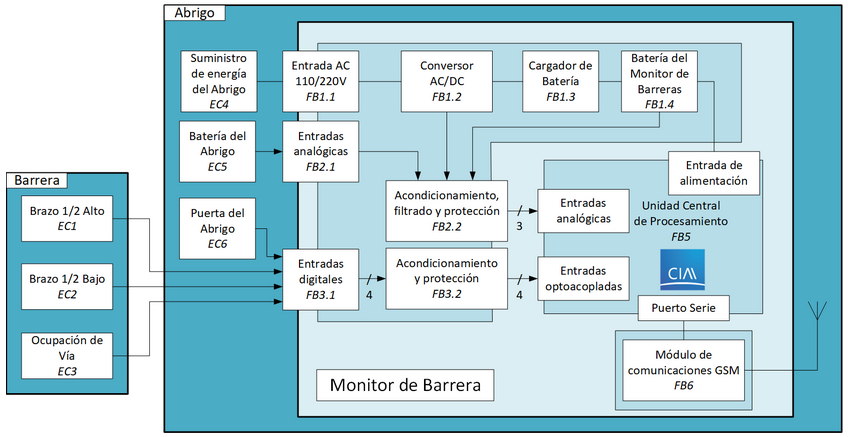
\includegraphics[width=1\textwidth]{./assets/diagBloques.png}
\caption{Diagrama en bloques del sistema}
\label{fig:diagBloques}
\end{figure}

\vspace{25px}

El tamaño de la tipografía en TODAS las figuras debe ser adecuado para que NO pase lo que ocurre acá, donde el lector debe esforzarse para poder leer el texto. Los colores usados en el diagrama deben ser adecuados, tal que ayuden a comprender mejor el diagrama, preferentemente en la gama de colores pastel.
\end{consigna}
